\section{The finite-size statement}
\label{sec:statement}

\begin{theorem}[Finite-size number-sector-incoherent passive separation]
\label{thm:main}
For the four-fold forrelation promise problem at $N=4096$, every protocol in $\classP$ with branchwise hard dose at most six has worst-case promised error greater than $1/3$, while a protocol in $\classA$ with branchwise hard dose six has worst-case promised error $81/256$. Therefore
\begin{equation}
\boxed{
\Dhard_{\classP}(4096)>6,
\qquad
\Dhard_{\classA}(4096)\le6.}
\end{equation}
The passive lower bound covers unrestricted classical feed-forward between fresh quantum batches satisfying Eq.~\eqref{eq:model-number-sector}. It excludes coherent quantum memory or coherent control carried between batches and coherence between different total signal photon-number sectors within a batch.
\end{theorem}

\paragraph{Claim grade.} Theorem~\ref{thm:main} is theorem-level. Its passive numerical input is an outward certificate, its adaptive extension is analytic with multiplier one, and its active upper bound is pointwise on every promised input.

\subsection{Numerical certificate}

The passive proof uses two conditioned hard laws $P_+$ and $P_-$. The following displayed upper bounds are rounded upward from the exact directed-arithmetic artifacts.

\begin{align}
P_{\mathrm{Perron}}
&\le 0.258744096385577223,
\\
P_{\mathrm{promise}}
&\le 0.002225128406630703,
\\
\TV(P_+,P_-)
&\le 0.260969224792207925.
\label{eq:statement-total}
\end{align}

The acceptance threshold used by the certificate is

\begin{equation}
\frac13-10^{-3}=0.332333333333333333\ldots,
\end{equation}

so the outward total retains the lower reserve

\begin{equation}
0.071364108541125408.
\end{equation}

For equal priors, the Bayes error is $(1-\TV)/2$, and Eq.~\eqref{eq:statement-total} gives

\begin{equation}
p_{\mathrm{err}}^{\mathrm{passive}}
\ge 0.369515387603896037
>\frac13.
\end{equation}

An average error lower bound over hard distributions supported on the two promise sets implies that every passive hard-dose-six protocol fails on at least one promised input.

\subsection{Reading the separation}

At dose six, the active error $81/256=0.31640625$ lies $13/768\simeq0.01693$ below the required error $1/3$. The passive hard-pair error is at least $0.369515387603896037$, which lies approximately $0.03618$ above $1/3$; because this is an average over promised inputs for an arbitrary protocol in $\classP$, at least one promised input has error no smaller than this average. Figure~\ref{fig:certificate} displays the certificate assembly and the two resulting decision-error statements on a common scale.

\begin{figure*}[t]
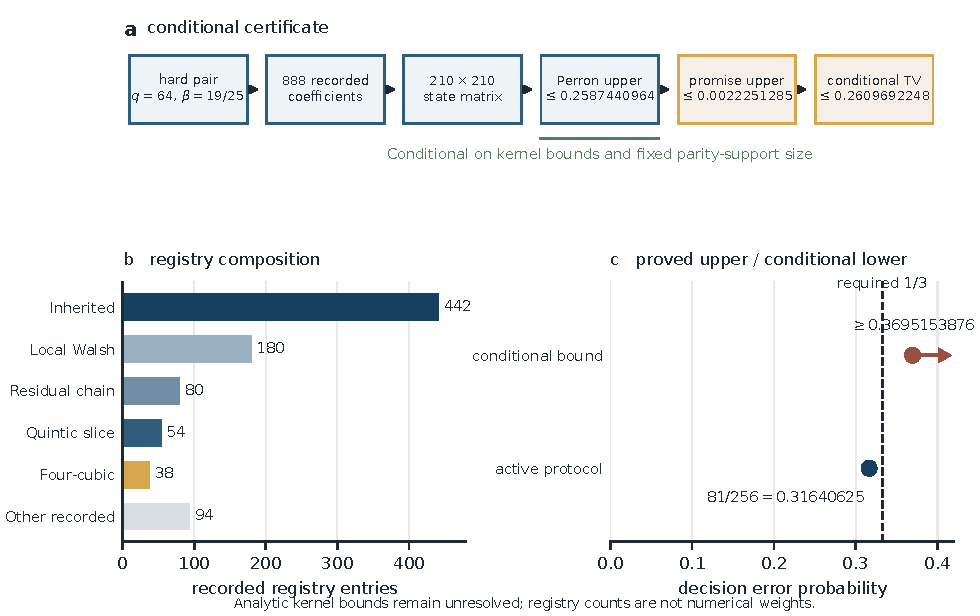
\includegraphics[width=\textwidth]{figures/passive_certificate.pdf}
\caption{Assembly of the number-sector-incoherent passive certificate and the resulting finite-dose separation. The 888 balanced arbitrary-correlated-law occurrence coefficients assemble the 210-state matrix, whose outward Collatz--Wielandt upper is $0.2587440964$; the normalized adaptive factorization contributes multiplier one, and promise conditioning contributes at most $0.0022251285$. The passive equal-prior hard-law error is at least $0.3695153876$, which implies a worst-case promised obstruction in the stated passive class, while the explicit active protocol has pointwise worst-case error $81/256$. Registry bar lengths count certified entries and do not measure their numerical contributions.}
\label{fig:certificate}
\end{figure*}

\subsection{Dependency structure}

The proof dependencies are ordered. The physical occurrence theorems establish arbitrary-correlated-diagonal coefficients for all balanced entries. The one-batch program rejects every unbalanced routing value, replaces each accepted coefficient by a strict rational upper, reconstructs the number-sector-block-diagonal 210-state nonnegative matrix with directed arithmetic, and certifies its spectral radius. The adaptive theorem factors the complete outcome tree into one normalized feature family, pulls temporal histories back to aggregate Fock occupations, and applies the same occurrence matrix to two independent normalized laws. Promise conditioning is paid once after the unconditioned comparison. The active upper bound uses a separate pointwise interferometric identity and does not depend on the passive hard distribution.
